\documentclass{article}
\usepackage{helvet}
\usepackage{enumerate}
\usepackage{amsmath}
\usepackage{amsfonts}
\usepackage{graphicx}
\usepackage{hyperref}


\title{BertonGan: a conditional GAN for performing various tasks}
\author{ Aaron Schindler, Herbert Wright }
\date{\today}

\begin{document}

% the title page
\maketitle
\pagebreak

% the introduction/background section
\section{Introduction}

\subsection{Problem Statement}

Given data $\mathcal D = (X, y)$ drawn from some unknown distribution
such that $X \in \mathbb R^{n_x \times d}$, and $y_i \in y$ is an "identity" or "style class"
of example $x_i$, we wish to define a function $\hat{f}$ such that we can take in
a "content" image and a "style" image and generate an image that is close to the "content" in distance,
but shares the same "style class" as the style image.


This is called style transfer and one common application is face swapping.
In this instance, our style classes are people's identities, and we are trying to, given one image,
project another image's person's face onto it.

% We wish to construct a network that can, given a few images of an unseen face,
% construct face images/deepfakes that are similar to that one, even if it has not
% seen that person before. \cite{lin2020using} is an example of face swapping, but without the
% few-shot learning of new faces.

% Deep learning is the traditional method of generating and detecting deepfakes \cite{nguyen2022deep}.
% While some computer graphics methods can be used, they lack the same ability
% of deep learning architectures to capture and learn complex functions efficiently.
% Because the images generated by deepfake architectures are very realistic, most
% humans are not able to distinguish between real and fake images. We can
% use a different (or same in some cases) models to learn the subtle differences
% between real and fake images, like differences in noise or counts of pixel colors,
% to effectively decide if an image is real or not.

\subsection{Generative Adversarial Networks}

Generative Adversarial Networks (GANs) were introduced by Ian Goodfellow \cite{goodfellow2020generative},
and are a common way to perform style transfer.
One such example is StyleGAN \cite{karras2019style}.
An example of a GAN being used for face swapping specifically can be found in \cite{lin2020using}.
Unfortunately, these GANs tend to require a lot of data and computation to train.


% the methods section
\section{Methods}

\subsection{BertonGan structure / Netorks}

Our Approach is two learn a metric of face/style classes via an encoder network,
then learn to encode image content with a seperate encoder, and then a decoder network which operates on both inputs.
We also define two different discriminator outputs; the first determines if the image is fake,
the second is conditioned on a latent vector from our face/style classes encoded space and determines if the image
belongs to that style class.
In short we have 5 different networks:

\begin{enumerate}
	\item Face encoder network: $f_F: \mathbb{R}^{n\times W \times H} \rightarrow \mathbb{R}^{h_f}$
	      \begin{enumerate}
		      \item Input: $n$ images of the same subjects face
		      \item Output: A latent representation of the subjects face
	      \end{enumerate}
	\item Image encoder network: $f_I: \mathbb{R}^{W \times H} \rightarrow \mathbb{R}^{h_I}$
	      \begin{enumerate}
		      \item Input: An image of a subjects face
		      \item Output: A latent representation of the image
	      \end{enumerate}
	\item Image decoder network: $f_G: \mathbb{R}^{h_F + h_I} \rightarrow \mathbb{R}^{W \times H}$
	      \begin{enumerate}
		      \item Input: Latent representations of a face and image
		      \item Output: A reconstructed image decoded from the latent features
	      \end{enumerate}
	\item 2 Discriminator networks: $f_D: \mathbb{R}^{W \times H} \times \mathbb{R}^{h_F} \rightarrow [0,1]^2$
	      \begin{enumerate}
		      \item Input: An image and a latent representation of a face
		      \item Output: Two probabilities (each of these probabilities has it's own corresponding network in practice)
		            \begin{enumerate}
			            \item Probability of being a fake image
			            \item Probability of being a different person than the faces encoded into the latent vector
		            \end{enumerate}
	      \end{enumerate}
\end{enumerate}

We generate our images by encoding our style image ($F_A$)
and our content image ($I_A$ or $I_B$ depending on its style class)
with our two different encoders, then feeding the output into
our image decoder network. Our discriminators use this as input.
A visual of the flow of the network is shown in figure 1
(circles denote networks and boxes are tensor inputs or outputs):

\begin{figure}[hbt]
	\centering
	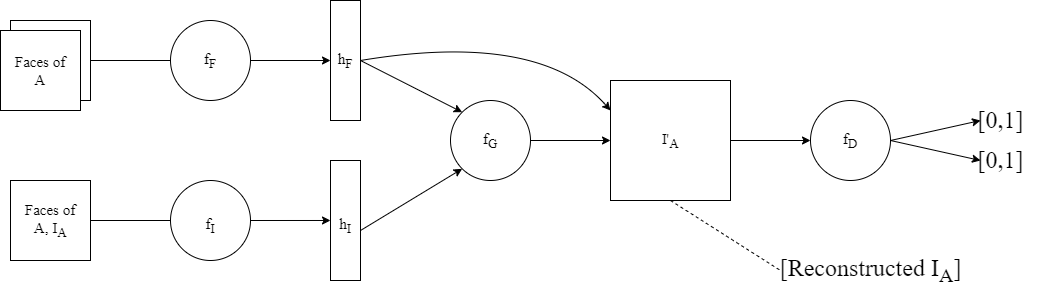
\includegraphics[scale=0.25]{images/OurNetwork.png}
	\caption{Figure 1 is a visual representation of our total network, comprising each of the four components above}
	\label{fig:my_label}
\end{figure}


\subsection{Training Procedure}

We propose using two datasets to train/test. The first is the built in MNIST dataset from the torchvision package \cite{deng2012mnist}. This dataset will allow us to experiment with our networks on a smaller scale, as the MNIST images are $28 \times 28$ images of numbers rather than people. The next step is to use the celebA dataset which is also built in to the torchvision package. Our original plan to use the MS-Celeb-1M dataset \cite{guo2016ms}
has been changed because the dataset is no longer publicly available. The celebA dataset comprises over $200,000$ images of faces, that are $178 \times 218$ in size.

Given a batch $\beta = (F_A, I_A, I_B)$, where $F_A = n$ faces of person $A$, $I_A = N$ other faces of person $A$, and $I_B = N $ faces of people other than person $A$, we will compute the following quantities:
\begin{enumerate}
	\item $h_F = f_F(F_A) \in \mathbb{R}^{h_F}$
	\item $h_I = f_I(F_B) \in \mathbb{R}^{N \times h_I}$
	\item $h_B = f_I(F_B) \in \mathbb{R}^{N \times h_I}$
	\item $I'_A = f_G(h_F, h_I) \in \mathbb{R}^{N \times W \times H}$
	\item $I'_B = f_G(h_F, h_B) \in \mathbb{R}^{N \times W \times H}$
	\item $(R_{A'}, C_{A'}) = f_D(I'_A, h_f) \in [0,1]^{N \times 2}$
	\item $(R_A, C_A) = f_D(I_A, h_F) \in [0,1]^{N \times 2}$
	\item $(R_{B'}, C_{B'}) = f_D(I'_B, h_F) \in [0,1]^{N \times 2}$
	\item $(R_B, C_B) = f_D(I_B, h_f) \in [0,1]^{N \times 2}$
	\item $D_A = \|I_A - I'_A\|$
	\item $D_B = \|I_B - I'_B\|$
\end{enumerate}

We will optimize $f_D$ by maximizing $R_A, R_B, C_A$ and minimizing $R_{A'}, R_{B'}, C_B$. We also optimize $f_F$ by maximizing $C_A, C_{A'}, C_{B'}$ and minimizing $C_B, D_A$.
Additionally, we optimize $f_G, f_I$ by maximizing $R_{A'}, R_{B'}, C_{A'}, C_{B'}$ and
minimizing $D_A, D_B$.
For stability purposes, we use a least-squares loss as proposed for GANs in \cite{mao2017least}
All parameters are optimized by using stochastic gradient descent.

After training, we will be able to use $f_F, f_I, \text{ and } f_G$ to perform face swaps or style transfer. We will then use $f_D$ to identify fake/real images generated using face encoding $h_F$. Additionally, we will use $f_F \text{ and } f_G$ to generate new images of an already learned face.



% the experiments section
\section{Experiments}

Code for all experiments can be found in our GitHub repo here:


\href{https://github.com/Herb-Wright/berton-gan}{https://github.com/Herb-Wright/berton-gan}

\subsection{MNIST Experiments}

We first trained on the MNIST dataset with defined networks that were not too far from the GANs we used in the notebook in class.
In the first BertonGan we trained ended up with saturated gradients in the discriminator1 network
(the one that predicts whether or not the image is fake).
After this, the generator was able to easily fool this, leading to fuzzy output images.
We trained this network for 50 epochs.
We show two different graphics in figures 2 and 3; the first is performing our version of style transfer
where the number of the image is the style class it belongs to,
and just some generated images from picking random content and style images.
All of the style and content images are from the test set and thus not seen before by the network.

Note that in figure 2, columns 1 and 4 are content, 2 and 5 are style (digit number), and 3 and 6 are the generated image.
The goal is for the third column's image to be "close" to the first column, with the same number as the second.


\begin{figure}[hbt]
	\centering
	\begin{minipage}{.5\textwidth}
		\centering
		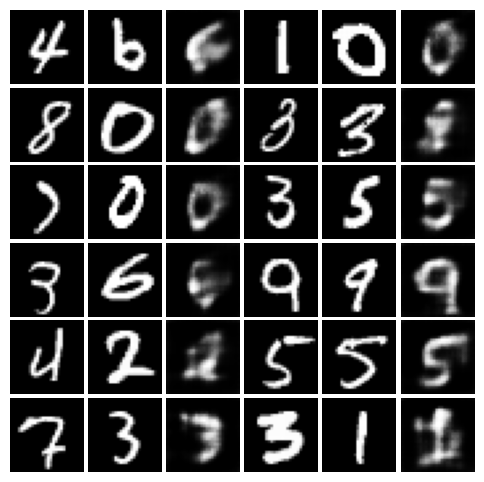
\includegraphics[width=.8\linewidth]{images/mnist_transfer_fuzzy.png}
		\caption{(a)}{Style transfer}
		\label{fig:sub1}
	\end{minipage}%
	\begin{minipage}{.5\textwidth}
		\centering
		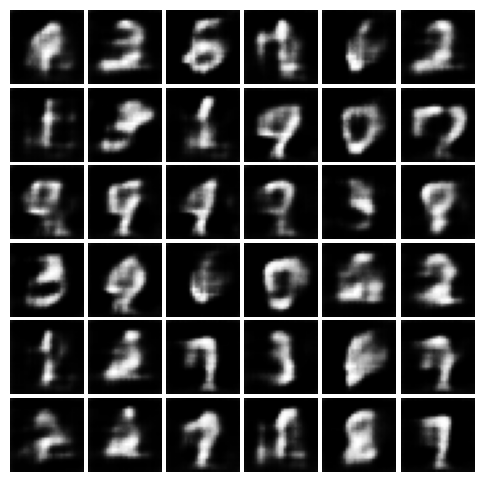
\includegraphics[width=.8\linewidth]{images/mnist_generated_fuzzy.png}
		\caption{(b)}{Generated images}
		\label{fig:sub2}
	\end{minipage}
\end{figure}

The gradients were being saturated because we had a sigmoid in the last layer of the network to output a probability.
We removed this activation, added two more layers to the network and retrained.
We used a slightly different procedure this time around;
we first trained the image encoder and decoder as an autoencoder for 5 epochs, then trained the whole network.
Figures 5, 6, 7 and 8 show this network at various epochs.
Figures 9 and 10 show, after 50 epochs, our version of style transfer and a sample of generated images similar to figures 2 and 3.
Each image used for content and style is from the test set as before


\begin{figure}[hbt]
	\centering
	\begin{minipage}{.5\textwidth}
		\centering
		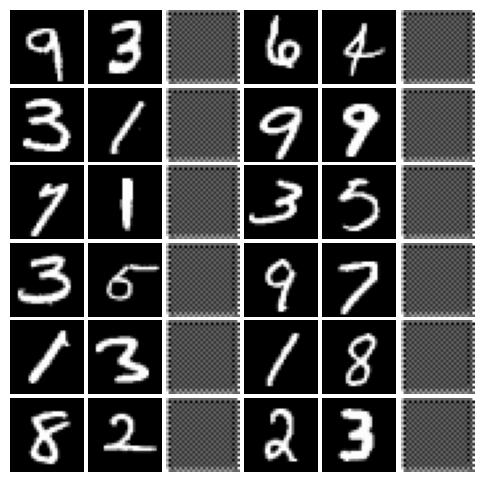
\includegraphics[width=.8\linewidth]{images/mnist_transfer_crisp_1.png}
		\caption{(a)}{1st epoch (random noise)}
		\label{fig:sub3}
	\end{minipage}%
	\begin{minipage}{.5\textwidth}
		\centering
		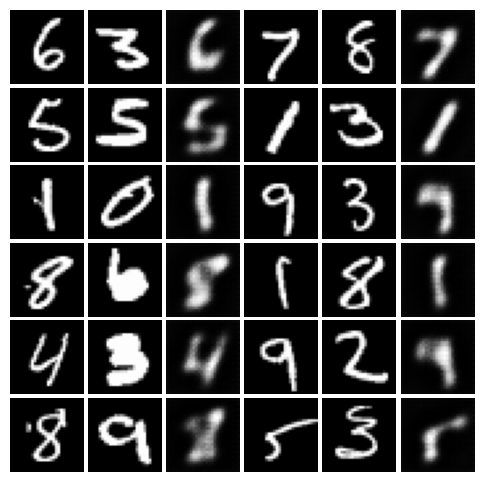
\includegraphics[width=.8\linewidth]{images/mnist_transfer_crisp_5.png}
		\caption{(b)}{5th epoch (autoencoder)}
		\label{fig:sub4}
	\end{minipage}
\end{figure}

\begin{figure}[hbt]
	\centering
	\begin{minipage}{.5\textwidth}
		\centering
		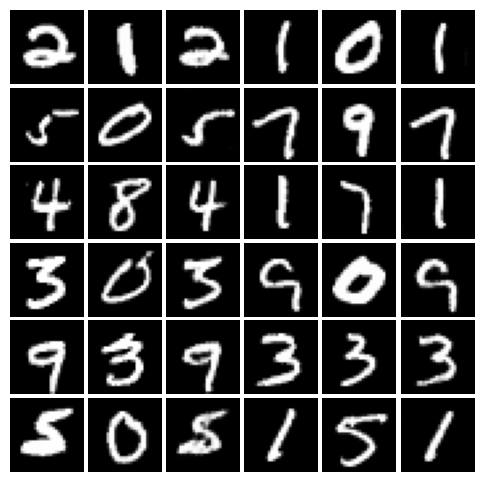
\includegraphics[width=.8\linewidth]{images/mnist_transfer_crisp_15.png}
		\caption{(a)}{15th epoch (no style transfer)}
		\label{fig:sub5}
	\end{minipage}%
	\begin{minipage}{.5\textwidth}
		\centering
		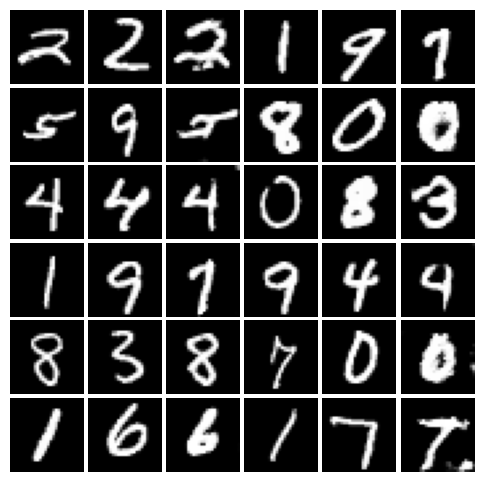
\includegraphics[width=.8\linewidth]{images/mnist_transfer_crisp_30.png}
		\caption{(b)}{30th epoch}
		\label{fig:sub6}
	\end{minipage}
\end{figure}



\begin{figure}[hbt]
	\centering
	\begin{minipage}{.5\textwidth}
		\centering
		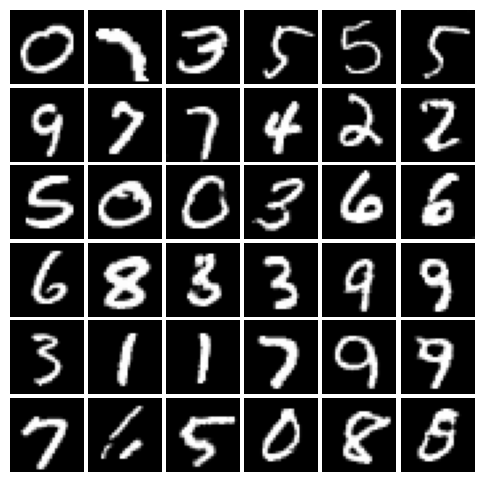
\includegraphics[width=.8\linewidth]{images/mnist_transfer_crisp_50.png}
		\caption{(a)}{Style transfer (50th epoch)}
		\label{fig:sub7}
	\end{minipage}
	\begin{minipage}{.5\textwidth}
		\centering
		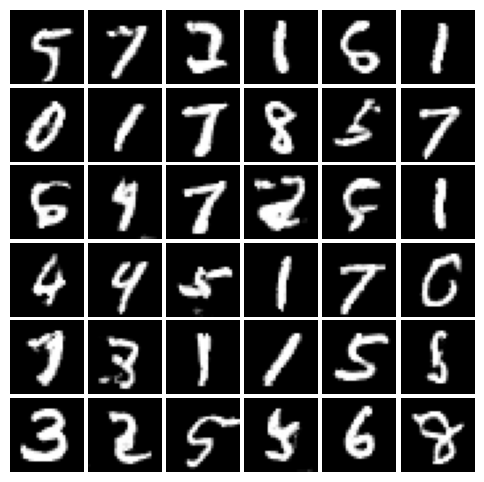
\includegraphics[width=.8\linewidth]{images/mnist_generated_crisp_50.png}
		\caption{(b)}{36 generated images}
		\label{fig:sub8}
	\end{minipage}
\end{figure}

\clearpage

We can evaluate our face/style metric space by performing classification on the MNIST test data in the following way:
first run through the training dataset and use the face encoder network to encode each digit,
then average the latent vectors for each style class (digits 0, 1, ..., 9).
Then, for each image in the test dataset, find the class whose averaged latent vector acheives the highest score from
the second discriminator network (the one that predicts if the image and latent vector belong to the same class).
Performing this procedure on the MNIST test images achieves $97$\% accuracy, suggesting an informative metric was learned.


Because we use latent dimension of 2 for our face/style encodings (encoding of the digit shown),
we can display a grid of how this value changes as you move throughout the latent space for a given image.
In figure 10, we encode the same image with the image encoder network then vary the latent face/style encoding vector.
The output is the similar images but with the number changing as you move in the latent space.

\begin{figure}[hbt]
	\centering
	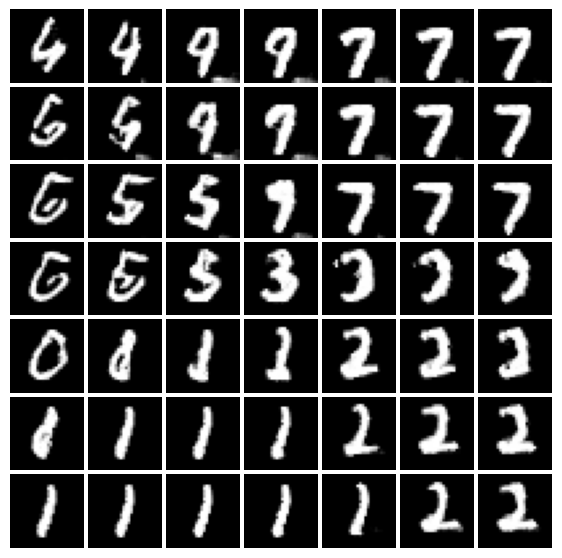
\includegraphics[scale=0.5]{images/mnist_latent_crisp_50.png}
	\caption{visualization of latent space}
	\label{fig:fig3}

\end{figure}


\clearpage

\subsection{CelebA Experiments}

% Unfortunately, because we spent more time on building/improving the MNIST dataset there was not enough time to adequately experiment with
% the celebA dataset. We do have the network partially built, a network that downsamples first in order to be more efficient since the data
% we are working with in the celebA dataset is much larger than MNIST.


% the conclusion/future work section
\section{Conclusion}

In conclusion, it is very clear that when generating deepfakes it is possible to perform style transfer via metric learning using GANs. One downside to
performing this operation was the amount of time and compute resources it takes to train the network. It takes roughly 10 minutes to train using cloud
computing resources such as google colab for just the MNIST dataset.
It took over 2 minutes for one epoch when trained on the CPU. Because of this, the celebA dataset presented an entirely new challenge since the
dataset size is much larger than MNIST.
When we tried to train on the CelebA dataset, it took roughly 27 minutes to complete one epoch.
It would be nice to see if there was some way to alter the structure of BertonGan or training procedure so that it didn't take quite as long.
Despite this, our MNIST experiments clearly show potential in style transfer via learning a metric.

	{\bf Future Work.} In another direction, diffusion models have grown in popularity for image generation \cite{croitoru2022diffusion}. It would be interesting to see if ideas from BertonGan could be translated into the diffusion model setting, where you still learn metric and condition your diffusion model on the metric space.


% We believe the future direction of this work is to build an efficient network for celebA by using downsampling in order to decrease the number of parameters
% that need to be computed at intermediate steps. An added difficulty of the celebA dataset is that becasue images are larger and more robust than that of MNIST
% we also believe that a deeper network will be required. The proposed solution will be to model a network like ResNet, which downsamples in intermediate blocks.
% This not only creates a deeper network, but the size is easily variable since blocks can be added to the model easily.

\pagebreak

\bibliography{sources}
\bibliographystyle{ieeetr}

\end{document}
